%% *************************************************************************
%%
%% This is a derivative work of the RIT Space Exploration Standard defining 
%% guidelines for content and formatting of project design documents.
%%
%% This document uses IEEEtran.cls, the official IEEE LaTeX class
%% for authors of the Institute of Electrical and Electronics Engineers
%% (IEEE) Transactions journals and conferences.
%%
%% *************************************************************************

%% *************************************************************************
% LaTeX REFERENCES
% ----------------
%   Intro to LaTeX: http://www.rpi.edu/dept/arc/docs/latex/latex-intro.pdf
%   Comprehensive LaTeX symbol list: http://tug.ctan.org/info/symbols/comprehensive/symbols-a4.pdf
%% *************************************************************************

% tell \LaTeX what kind of formatting to use
\documentclass[conference]{IEEEtran} % http://www.ctan.org/pkg/ieeetran
\usepackage{graphicx} % enable toolbox for embedding figures and pictures
\usepackage{siunitx} % enable package for easily formatting units
% how to use hyperref: http://www2.washjeff.edu/users/rhigginbottom/latex/resources/lecture09.pdf
\usepackage[T1]{fontenc} % change text encoding to make it more crisp
\usepackage{etoolbox} % enable conditionals for help text
\usepackage{tabularx} % add stretchy cells and autosizes to tables
\usepackage{booktabs} % make beautiful tables!
\usepackage{hyperref} % enable package for cross-referencing figures, sections, references etc.

% set title. choose something as descriptive and precise as possible. Descriptive > sounding cool. remember this!
\title{SDL-IREC Competition Payload: SPEXTRO}

\author{
  % List the authors of the design document. The Champion should go first.
  % The \$~\$ markers tell \LaTeX{} to treat the text inside to be treated as a math expression. This way you can use operators like \textcaret{} to place characters as superscripts.
  % Some \LaTeX{} templates handle the author block in different ways. For example, the \href{http://www.worldscientific.com/worldscinet/jai}{Journal of Astronomical Instrumentation} requires the authors' addresses and emails to be included as well.
  % The \textbackslash{}thanks command puts the contents inside those brackets in a footnote at the bottom of the first page. Technically speaking, \textbackslash{}thanks is just a specially formatted footnote.
  % IEEE also has a ``long form'' author block for many authors. Check here for more information:
  % \url{https://tex.stackexchange.com/questions/156523/multiple-authors-with-common-affiliations-in-ieeetran-conference-template}
  % Read here for a more advanced options to modifying footnotes in the author block:  \url{http://tex.stackexchange.com/questions/826/symbols-instead-of-numbers-as-footnote-markers}
  %   Here, we use the IEEE long-form author block.
  \IEEEauthorblockN{% This block is for author Names.
    James~Parkus\IEEEauthorrefmark{1},  %the number in the bracket is a reference number to identify this footnote. \LaTeX will figure out what symbol to put there.
  }
  \IEEEauthorblockA{% This block is for the author Affiliations, aka department and university
    RIT Space Exploration, Rochester Institute of Technology \\ %\\ starts a new line
    Rochester, N.Y. \\
    Email:
    \IEEEauthorrefmark{1}jep7631@rit.edu
  }
  %%   Below, we use the short-form author block and basically hack it to suit our needs.
  % Philip~Linden$^{*\dagger}$%
  %   \thanks{$^{*}$Project Champion}%
  %   \thanks{$^{\dagger}$BS/MEng '17, Mechanical Engineering},
  % Austin~Bodzas$^{\ddagger}$%
  %   \thanks{$^{\ddagger}$BS '19, Computer Science},
  % Drew~Walters$^{\S}$%
  %   \thanks{$^{\S}$BS '18, Mechanical Engineering Technology},
  % T.J.~Tarazevits$^{**}$%
  %   \thanks{$^{**}$BS '19, Game Design \& Development}%

  %%   If there are many authors, consider using symbolic, numeric (aka arabic),  alphabet footnotes or a combination thereof.
  %% the recommended order for symbolic footnotes is
  %%   (1) asterisk        *   *
  %%   (2) dagger          †   \dagger
  %%   (3) double dagger   ‡   \ddagger
  %%   (4) section symbol  §   \S
  %%   et cetera. For higher counts, use 2x symbols (1)-(4) (i.e. (5) two asterisks **). Keep cycling through (1)-(4) using 3x, 4x, and so on.
  %%   Note that these symbol codes work in math mode and text mode.
  %%   There are ways to make LaTeX do this for you, but it is more advanced and not entirely necessary, especially for short author lists. Not worth the hassle, in my opinion.
}

% Initial setup is over, start building the document itself
\begin{document}
\maketitle%
% correct bad hyphenation here, separated by spaces
\hyphenation{explor-ation}

\begin{abstract}
The purpose of this experiment is to prove that understanding protein folding in zero-gravity could be conducted in a CubeSat form factor. This project will attempt to put this 
concept to work in a CubeSat that will be launched in a sounding rocket to 30,000 feet made by RIT Launch Initiative. Successfully completing this experiment will raise the Technology Readiness Level to which can be adequetly justified for a CubeSat mission to orbit.
      % The abstract is a brief summary of the design document. Typically it includes the purpose of the design document, key goals or objectives, and justifications.
      % Be sure not to confuse the abstract with the introduction.
      % It is easiest to write the abstract after the rest of the paper has been written.
      % That way you can choose key information from the sections that you've already completed and string them together in the abstract.
      % Consider the abstract to be your elevator pitch to anyone reading this design document.
      % What are they reading?
      % What is the goal?
      % Why is it worth my time?
      % The abstract is what will show up in Google results and other search engines, and what people will read when they are deciding what is worth their time and brain power.
\end{abstract}
% HELPFUL HINTS
% 1. If you get the linter warning ``Command terminated with space.'' when using a \command try placing ``%'' or ``{}'' immediately following the command.
% 2. For proper quotes, begin with `` and close with ''. For single quotes, use '. Double quotes characters copied from Word or Docs (") will show up as weird characters.

% The sections included here are required. Additional sections and subsections may be added as necessary.
\section{Introduction}
\label{sec:introduction}
  % The introduction is a place to give background and context before diving into the subject matter.
  % Establish context for the work you are about to propose and the main ideas of the proposition itself.

The project purpose is to create a 3U CubeSat payload which houses a protein spectroscopy experiment and fly on a sounding rocket in the 2020 IREC. The goal of this project is prove that 
this experiment can accurately detect protein folding after a rocket launch and in harsh ambient conditions. The success of this experiment will be a "proof-of-concept" of the protein spectroscopy
experiment conducted in a CubeSat form factor. This project will be launched on a rocket that RIT Launch Initiative will make to go to 30,000 feet. This rocket will be launched during the 
Intercollegiate Rocket Engineering Competition in 2020 (IREC 2020). 

\section{Primary Objective}
\label{sec:primary-obj}
  % At the end of the day, whether the project ``succeeds'' or ``fails'' is judged against the objectives it sought to meet.
  % Note that results that contradict expectations/hypotheses are not failures if the scientific \& engineering methods are followed along the way.
  % Sometimes our expectations are wrong and that can be just as successful as getting data we thought we'd see.
  % What matters are what questions you intend to answer.
  % This is the main purpose or main goal the project hopes to achieve.

The primary objective of this payload is a proof-of-concept mission aimed at understanding if protein spectroscopy can be performed in a CubeSat form factor. The experiment
is a scientific process in which proteins are analyzed to understand if they folded under free-fall conditions. Due to the mechanics of rocket flight, free fall (similar to that
of satellite orbit) is impossible to attain. Hence, the mission is focused on fitting this experiment in a 1U section of a larger 3U form factor and proving the experiment can be 
successfully conducted in such conditions during descent after jetison. 

\section{Benefit to SPEX}
\label{sec:benefit}
% One of the core values of SPEX is to provide opportunities for academic and professional growth for its members,
% and to challenge them with interesting projects.
% In this section, explain how the project would benefit SPEX members as students,
% space enthusiasts, and young professionals.

This project is an ordeal, as is rocketry. Launching payloads on rockets requires rigorous work to understand the intense vibrations and physical conditions as well ensuring the 
payload can survive the launch and function properly afterwards. The engineering is very involved, right down to the heads of the bolts (smallest details). How does everything 
fit together? Where do the wires go? These are but a few of the questions this team will learn to answer. The last IREC team gained a lot of experience in this area and collected 
and recorded it in a final document called \textit{SPEX IREC 2018 Final Report} located in the \textit{SPEX Google Drive: Workgroup Archive}. The next team will learn all these lessons intensively and painfully 
and will inevitably add to this list of lessons learned. While this may sound negative, it is exactly the opposite. Through the head scratching and confusion comes new ideas and engaging, 
novel, and rewarding experiences. This project would be massively beneficial to the students involved and thereby the rest of SPEX when these students move onto greater things. 

\section{Implementation}
\label{sec:implementation}
  % What path do you anticipate the project to take?

There are a few important points that must be understood to understand the scope of this project. 

This project will be a joint effort with RIT Launch Initiative. They are providing the launch vehicles and we, the payload. We are doing this together to compete in the 
Intercollegiate Rocket Engineering Competition in 2020. It must be understood that the project schedule will have a dependence on the LI rocketry team schedule. For instance, 
test fitting with their SABOT with require the mechanical footprint of the structure to be designed and fabricated. To this end, it is worth the time to obtain a working structure 
manufactured by the end of the Fall semester. This will serve as a initial integration structure. A important lesson learned from Hyperion was there were many integration 
issues that could have been sorted out far beforehand if there was a test-fit opportunity. This structure will not be the final design but an important stepping stone for the 
rest of the project. The manufacturing will be worth-while training for the engineers when it comes time for the manufacturing of the flight structure. 

The team leader will be the role of system engineer and lead designer for the project. The lead engineer will take the role of system engineer and lead designer for the structure.
The project scientist will be in charge of getting the experiment working. That includes all of the engineerind, data analysis, and other science that must go into the experiment.
A team hierarchy is proposed in \autoref{fig:hierarchy}.

\begin{figure}
  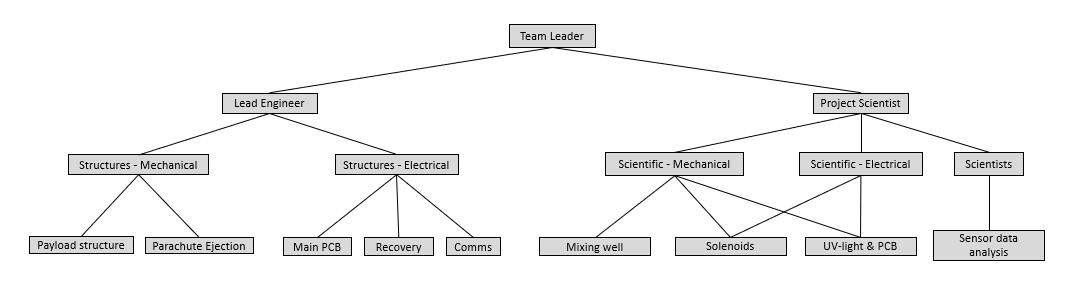
\includegraphics[width = \columnwidth]{figs/team_hierarchy.png}
  \caption{The team hierarchy is created based upon NASA-led missions. While the structure is not identical it hits the key figures, team leader (principal investigator), lead engineer
  (system engineer), and project scientist is the same. This structure has been adapted to help the team function well and achieve the goals of the project.}
  \label{fig:hierarchy}
\end{figure}

\subsection{Deliverables}
\label{subsec:deliverables}
  % When all is said and done, what will you have to show for it?
  % Examples: Hardware, software, poster, ImagineRIT demo, presentations, technical papers...

  The final product of this project will be a flight payload with a fully functional and LI independent communications system, recovery system, protein spectroscopy experiment, and parachute ejection 
  system. The communications system will have an APRS and GPS that operate on different frequencies than LI as to not interfer. The GPS and APRS must have sufficient battery life 
  to support extensive time from rocket integration to launch (~2 hrs) and then recovery (~12 hours). The recovery system will have a buzzer and maybe LEDs, this was discussed 
  but not executed on the 2018 IREC payload. The protein spectroscopy experiment will have the full mixing system with the UV-light and sensor, the data from which will be stored 
  locally and analyzed after recovery. The parachute system will likely include a Peregrine CO2 system, identical to the one used on Hyperion. 

\subsection{Milestones}
\label{subsec:milestones}
  % Be as detailed as you can, but it's okay if there are unknowns.
  % At the very least, specify how many semester you expect the project to take until it reaches completion.

  One point that the author must be clear on:

  \textit{It is my personal opinion that any attempt to achieve perfect free-fall to create the essential experiment upon the limitations of this project is time that 
  could be better spent creating a strong design and achieving a solid scientific result that can serve as "Proof of Concept". This idea will then be green-lit for a future 
  CubeSat proposal and this team could lay the bedrock upon which that CubeSat can be built.}

  The first goal of this experiment should defining the mission statement and success criterion. This will create a clear path forward for the engineering and science teams.
  Then the mechanical-science team should strive to create a functional experimental setup. This will be very important due the high complexity. They must first create an initial 
  model with a mixing well, solenoids, protein, and saline. They should first work to attain a good mixing of protein and saline. Then go onto the UV-light and sensor integration and testing. 
  Approach it one step at a time solving the problems with each one, meanwhile the structures team will work on developing an initial manufacturable model.

  The initial manufacturable model must be complete by Winter break to stay on a good track. There is enough known information about the sizing of the experiment and other components 
  to make a rough integration scheme. This assembly should favor modularity in the sense that things will change and it should be able to accomodate those changes. An idea would be 
  to create a small structure out of 80/20 (80/20 makes very small structures that will can accomodate the size restrictions). This would allow ease of access and re-positioning. 
  The goal of this model is to fully understand where everything will be placed including the wires. \textbf{An important lesson learned from Hyperion was understanding wire layout is 
  essential for integration. There was much work that went into strain relief of tightly packed wires from batteries and limit switches. The limit switches presented a difficult problem 
  in which their wires were protuding normal to the walls of the CubeSat and the extremely close proximity of the Main PCB meant those wires needed to do a 90 deg bend within an extremely 
  tight radius. This could have avoided with properly planning and time for integration studies.}

  There will also be two electrical teams, one dedicated to the scientific payload development and the other dedicated to comms, parachute ejection system, and Main PCB design. It is 
  recommended that the Main PCB be designed and ready for fabrication (WITH SPARES!) by the end of January. It will take a month to get all the parts and then a few weeks to get it fully populated. 
  The scientific payload team will work the mechanical engineers to create a functional experiment by the end of the Fall semester (recall: this is not scientifically functional, just mechanical and 
  electrically). 

\begin{table}[hb!]
    % the "h" in these brackets tells LaTeX to put the table Here. Try [t] for top and [b] for bottom,
    % or [hbp] for "here, or if you can't do that put it at the bottom of the page, or if you can't do that put it on its own page.
    % Here we've also used an "!" to yell at LaTeX to DO THIS OR ELSE!
    \caption{Notional timeline of Project Milestones.}
    \centering
    \begin{tabular}{@{}cll@{}}
    % the letters here ^^^^ designate the columns.
    % (l=left align, c=center, r=right align)
    % the weird @{} thingies tell LaTeX to not have left-right padding between cells
    % so cells butt up right against the edge
    \toprule
    Phase & Task & Duration \\
    \midrule
    1 & Mission Statement \& Success criterion & 1 week \\
    2 & Team leadership assortion & 1 week \\
    3 & Design and development & 6 weeks \\
    4 & Initial manufacturing & 4 weeks \\
    5 & Documentation update & 1 week \\
    6 & Design iterations & 4 weeks \\
    7 & Critical Design Review & 3 weeks \\
    8 & Final design iterations & 2 weeks \\
    9 & Flight manufacturing & 3 weeks \\
    10 & Flight integration and full system testing & 4 weeks \\
    11 & Launch and project review & 4 weeks \\
    \bottomrule
    \end{tabular}
\label{tab:short-example}
\end{table}

\section{Externalities}
  % Things not directly related to the work or outcomes, but related to the project as a whole.
\subsection{Prerequisite Skills}
  % Which skills do team members need to have before work can start (not including skills that will be learned ``on the job'')?
There are a few positions that will need to be held by experienced engineers/scientists to maintain an appropriate schedule. These positions are; team leader, project scientist, and lead 
engineer. The team leader should have previous project experience and preferrably system engineering experience, the project scientist should have previous project experience and experience with experimentation in their respective field 
of study, the lead engineer should have system engineering and past project experience and a strong handle of basic engineering fundamentals in their respective field. 

The people working under these personel do not have any knowledge or experience prerequisites. According to their field of study they should be taught the fundamentals early in the project 
timeline as to not cause schedule slip later on due to lack of experience. 

By the end of this project mechanical engineers should have more experience with Computer Aided Design, system fabrication, and system integration. The electrical engineers should have more 
experience in radio frequency analysis, location tracking (GPS, APRS), and PCB design and fabrication. Scientists (physicists, biologists, .etc) should have a stronger handle on designing and conducting 
experiments as well as analyzing the data and reporting it in a paper format. 

\subsection{Funding Requirements}
  % Estimate costs that would be needed to meet objectives.
The Hyperion payload required \$3000 to design, fabricate, integrate, and fly the payload. However, since this was the first project SPEX had undertaken of such a magnitude, the budget was 
used non-optimally (money was spent on items that it did not need to be). Learning from this experience a more accurate budget for the project can be estimated at \$2000. 

The structure is a 3U CubeSat. Assuming the materials are similar to the previous payload (safe assumption since the design will be off the Hyperion structure), it will cost about \$400. 
However, since this structure may change and require more materials, the price is safely approximated at \$600 for the structural engineering side of the project. 

The parachute ejection system will likely be the peregrine CO2 cartridge flight-heritage mechanism. This worked well for two separate launches for Hyperion (test launch in May and flight in June 2018). 
This system costs \$180, with additional cartridges this cost will be estimated at \$220. We already have a parachute and the material for the canister. 

The protein spectroscopy experiment has many 3D-printed mechanical parts which are very inexpensive. The main cost of this experiment will be the battery to run the solenoids, the solenoids, 
the protein, and the special material for the mixing well. The experiment will be given a budget of \$400 to develop the flight-ready assembly. This is on the higher end for cushion in case 
the material selection takes many different specimens to perfect. This is a complicated matter and was the subject of much research and testing in the Spring of 2019. Since the mixing well 
requires an unknown ratio of flexibility to strength, it is difficult to deduce the correct material from datasheets. The proteins are bovine and cost \$60. The solenoids have not been 
chosen, but based off testing completed in Spring 2019, they will cost about \$30 - \$40 each. A battery could cost up to \$50, the power requirements for the solenoids are not high but there 
will be redundency for long wait times. 

The electrical systems will be given a budget of \$700. 

\subsection{Faculty Support}
  % Identify faculty that will be involved (or would need to be involved) to meet objectives.
  % Note that if a professor is the Principal Investigator (P.I.) for a project, there still needs to be a student as the SPEX Project Champion.
We will require faculty support for funding and recruiting. Dr. Barbosu will be able to help the IREC team reach out to funding organizations to raise money for the project. There should also be 
opportunities for RIT funding or SEDS funding during the fall semester. 

The mechanical engineering department for KGCOE (Kate Gleason College of Engineering) is willing to send out emails to the entire engineering student body for us (probably once a semester). They 
do this to raise awareness of KGCOE projects that students can join. This will be done for the IREC group to recruit mechanical, electrical, and computer engineers. 

\subsection{Long-Term Vision}
\label{sec:vision}
The long term vision of this project is to enable a CubeSat to carry this payload into space to complete the experiment. This project will prove the experiment can be done in flight conditions. 
The payload will need to hold together and operate after intense launch vibrations and harsh ambient conditions. It is likely, based of preliminary talks with LI, that they will be launching this 
payload to 30,000 feet. At this altitude air is sparse and pressure and temperature is low. Conducting the experiment in these conditions is a strong indication this is a feasible experiment. 

\section*{Acknowledgements}
The author would like to thank Dr.~Bill Destler and Rebecca Johnson for being exemplary humans, Anthony Hennig for founding RIT Space Exploration, and all the SPEX members that continue to invest their time and energy into the pursuit of space exploration.

%\bibliographystyle{IEEEtran}
%\bibliography{sample-with-examples}

%\onecolumn
%\appendices{}
%\section{Project Life Cycle}


\end{document}
